% -*- Mode:TeX -*-
% TODO Try using ACM SIGCHI two-column layout
% TODO Need to make sure verb tense is consistent. Sometimes I use future and sometimes present.

%% The documentclass options along with the pagestyle can be used to generate
%% a technical report, a draft copy, or a regular thesis.  You may need to
%% re-specify the pagestyle after you \include cover.tex.  For more
%% information, see the first few lines of mitthesis.cls.

\documentclass{chi2011}
\usepackage{times}
%\copyrightnotice{This work is licensed under a Creative Commons Attribution 3.0 Unported License}
\usepackage{graphicx}
\usepackage{ucs}
\usepackage[utf8x]{inputenc}
\usepackage[pdftex]{hyperref}
\usepackage{color}

\hypersetup{%
pdftitle={Designing for Remixing: Supporting an Online Community of Amateur Creators},
pdfauthor={Andres Monroy-Hernandez},
pdfkeywords={remixing, online communities},
bookmarksnumbered,
pdfstartview={FitH},
colorlinks,
citecolor=black,
filecolor=black,
linkcolor=black,
urlcolor=black,
breaklinks=true,
}
\newcommand{\comment}[1]{}
\definecolor{Orange}{rgb}{1,0.5,0}
\newcommand{\todo}[1]{\textsf{\textbf{\textcolor{Orange}{[[#1]]}}}}

\pagenumbering{arabic}  % Arabic page numbers for submission.  Remove this line to eliminate page numbers for the camera ready copy

% add bibliographic stuff 
\usepackage[round]{natbib}
%%Prefatory material
\bibliographystyle{apalike}
%\bibliographystyle{acmnocaps}
%\bibliographystyle{acm-sigchi}
\def\citepos#1{\citeauthor{#1}'s (\citeyear{#1})}
\def\citespos#1{\citeauthor{#1}' (\citeyear{#1})}

%% This bit allows you to either specify only the files which you wish to
%% process, or `all' to process all files which you \include.
%% Krishna Sethuraman (1990).

% andresmh: commenting this out will ask you to manually enter which files you need to compile
%\typein [\files]{main}
%\ifx\files\blank \typeout{Including all files.} \else \typeout{Including only \files.} \includeonly{\files} \fi

\begin{document}
\special{papersize=8.5in,11in}
\setlength{\paperheight}{11in}
\setlength{\paperwidth}{8.5in}
\setlength{\pdfpageheight}{\paperheight}
\setlength{\pdfpagewidth}{\paperwidth}
\toappear{Thesis proposal submitted to the Program in Media Arts and Sciences, School of Architecture and Planning, in partial fulfillment of the requirements for the degree of Doctor of Philosophy in Media Arts and Sciences. \\This work is licensed under a Creative Commons. Attribution 3.0 Unported License} 
%%Formatting commands
%\setlength{\parindent}{0pt} %Full block style
%\setlength{\parskip}{11pt} %Assumes 11pt type
\hfuzz2pt % Don't bother to report over-full boxes if over-edge is < 2pt
%%Prefatory material
%\bibliographystyle{apalike}
%\bibliographystyle{acm-sigchi}
\input{acm-cover}
\input{acm-abstract}
%\keywords{put author keywords here} 
%\category{H.5.2}{Information Interfaces and Presentation}{Miscellaneous}[Optional sub-category]
%\terms{
%  See list of the limited ACM 16 terms in the instructions, see http://www.sheridanprinting.com/sigchi/generalterms.htm.
%}
%%readers.tex
%Readers page for AYB PhD thesis

% Provides a signature page for secondary readers on a thesis. Title info
% is gathered from the title page, and readers can be added below.
% Media Lab requires this. [AYB]
\reader{Yochai Benkler}{Berkman Professor of Entrepreneurial Legal Studies}{Harvard University}
\reader{Robert C. Miller}{Associate Professor of Electrical Engineering and Computer Science}{MIT Computer Science and Artificial Intelligence Laboratory}

\readerpage

%\cleardoublepage

%\pagestyle{plain}
%%Main body (chapters)
%\setlength{\parskip}{0pt} %Assumes 11pt type
%\begin{spacing}{1}
%\input{contents}
%\end{spacing}
%\setlength{\parskip}{11pt plus3pt minus3pt} %Assumes 11pt type
\chapter{Introduction}

In recent years, there has been an explosion of online communities where people share their ideas and creations.
Participants of these communities not only share their own work, they also remix, re-create, remake, re-tweet, fork, sample, mash-up, edit or appropriate other people's work to produce derivatives or remixes that are shared back to the community.
Previous work has described how these communities and the activities they support, have far-reaching implications for the way cultural and economic production work.
In this dissertation proposal, I outline a research framework to examine the design and usage of an active online remixing community built to engage young people in social production and creative learning.

Online remixing communities span a wide range of creative endeavors, there are communities for sharing and remixing 
\emph{code} (for instance, GitHub and Sourceforge),
\emph{articles} (for instance, Wikipedia and Wikia), 
\emph{videos} (for instance, YouTube and Vimeo), 
\emph{images} (for instance, Flickr and DeviantArt), 
\emph{status updates} (for instance, Twitter and Facebook),
\emph{music} (for instance, ccMixter and IndabaMusic),
and even the design of \emph{physical objects} (for instance, Ponoko and Etsy).
In this dissertation, I focus on the Scratch Online Community, a website developed to enable amateur creators, especially children aged between eight and sixteen, to share and remix animations and video games.
I plan to, first, describe the motivations and socio technical infrastructure of the Scratch website, then examine how people have used the website to collaborate with others through remixing and how the design has influenced these activities.

\chapter{Background}

I build on existing work that places remixing in new forms of cultural and economic production \citep{benkler_wealth_2006,jenkins_convergence_2006,manovich_remix_2005,sinnreich_ethics_2009}, and describes some challenges that remixing poses to our existing legal and moral assumptions \citep{lessig_remix:_2008, posner_little_2007}
Inspired by existing learning theories, for example \citet{lave_situated_1991}, I investigate remixing as a legitimate form of participation in a social learning environment.
Furthermore,  I build on the work that advocates remixing as a new media literacy skill \citep{ito_hanging_2010, jenkins_confronting_2009, livingstone_taking_2008, perkel_copy_2008}.
I look at the implications of remixing for the design of social computing systems by connecting to existing human-computer interaction research on systems for remixing and sharing videos \citep{diakopoulos_evolution_2007}, images \citep{seneviratne_policy-aware_2009}, music \citep{cheliotis_analysis_2009} and hypertext \citep{viegas_studying_2004}.

\section{The Scratch Online Community}

%TODO: once settled with layout, make sure it does not use a full page just for this image
\begin{figure}
\centering
\includegraphics[width=3.25in]{figures/websitehomepage.png}
\caption{The home page of the Scratch website}
\label{fig:websitehomepage}
\end{figure}

The empirical setting for this work is the Scratch Online Community, a website (Figure~\ref{fig:websitehomepage}) I conceived and developed over the past four years in collaboration with others at the Lifelong Kindergarten research group, for this and other lines of research.
The website allows anyone, especially young people between ages eight and sixteen, to share their animated stories, interactive art, and video games. Participants use the Scratch programming environment, a desktop application, to create or remix projects by putting together images, music and sounds with visual programming command blocks \citep{resnick_scratch:_2009}.
Projects range from interactive greeting cards, physics simulations, animations of popular songs to homemade video games, just to name a few.  

Scratch projects are organized in sprites (e.g. a character in a game).
Each sprite has a set of ``costumes'' or images that represent its different visual states, for example, a sprite of a bird flying could have multiple costumes, each one representing the different positions of the wings. 
Sprites can also have sounds associated to them, these sounds can be either recorded with the microphone or imported from the hard creator's hard drive. Finally, sprites' behavior is controlled by ``scripts'' which are stacks of visual programming blocks. 

In my dissertation, I plan to document in detail the motivations that led to the design of the Scratch website as it is now and the various iterations that it went through as a result of internal and user-driven demands and participation patterns.
I expand on the tight relationship between the technical capabilities of the website and the social dynamics that it supported or intended to support.
I take a critical look at how the original goals of the community were or were not achieved and in what ways that happened. 
I narrate scalability challenges with the technology and moderation of the community.
In the following two sections I provide a glimpse of this.

More broadly, I try to tackle questions such as: How was the culture of sharing seeded and maintained in a public space? What were some important incidents that changed policies or architecture? How did the architecture and management of the site influence the culture of the site and how did users help shap this? 
Was it the design of the space or the work of users to create the culture?
 What were the lessons learned along the way by administrators? What kinds of learning outcomes were achieved?
To answer some of these questions, I primarily rely on participant observation data, experiences collected during the three years and I support these arguments with descriptive statistics and case studies.


\subsection{Motivations}

From its start \citep{monroy-hernandez_scratchr:_2007,monroy-hernandez_empowering_2008}, I set the goal for the Scratch Online Community as to give creators access to 
1) a \emph{network of peers} that functions as an audience and as potential collaborators and,
2) a \emph{repository} of inspirational creations that can be creatively appropriated by anyone.

More broadly, the Scratch Online Community was created with the idea of supporting a Community of Practice around Scratch where novices and experts would come together,  in the spirit of Papert's Samba school's metaphor \citep{papert_mindstorms_1980}.

Additionally, the idea of the Scratch Online Community was conceived under the umbrella of embodying the ethos of Participatory Culture of empowering people to become producers rather than just consumers of media.

Last, the Scratch Online Community was motivated to support the various iterative stages of the creative process \citep{resnick_sowing_2008}, namely:
Supporting creators' \emph{imagination} by giving access to a pool of inspirational projects and ideas; supporting \emph{creation} by allowing people to reuse and remix; supporting \emph{play} by letting people interact with others and their creations within a community; supporting \emph{sharing} by allowing people to easily upload their creations to the platform; supporting \emph{reflection} by providing a space to receive comments and discussion forums for more in-depth discussions.

\subsection{Sociotechnical Infrastructure}
The Scratch website platform, called ScratchR, is broadly composed of the following components: 

\begin{enumerate}
\item A repository of projects and metadata. Projects can be downloaded by anyone, modified and re-uploaded to the website as a remix. Each project has its web page where it is displayed and where people can interact with it and other people. 

\item A social network consisting of profile pages and unidirectional friendship connections. Profile pages list the friends, projects and ``favorited'' projects for each user with his or her avatar image and the Country of origin (all self-reported data).

\item Social features for interacting with people's creation such as commenting, tagging, ``loving'', ``favoriting''.

\item Galleries, which are pages where people can group projects and talk about them. It is important to note that galleries have been repurposed by the community as group spaces where people collaborate to create projects or use it as a space to talk to one another or play Role Playing Games.

\item Discussion forums where community members help one another with technical problems, find collaborators and talk about non-Scratch related activities that foster a sense of community on the website.

\item External services supported by an API\footnote{API stands for Application Program Interface. In ScratchR, they are a set of web-accessible functions that let people retrieve and submit data such as login authentication and information about projects.} such as a website where people can link projects or a Wiki where people can document their experiences with Scratch and the community.
\end{enumerate}

The website runs on a hybrid model for moderation that combines user-driven moderation through flagging and appointed moderators working in parallel with a full-time staff member and other part-time ones that review the flags and ensure that the social dynamics are kept as civil as possible. 
This model has allowed for scaling the community management at a relatively low cost, however, much of the architecture and software development during the three years has been put into mechanisms for preventing antisocial behavior.

Three years after its official release, the Scratch Online Community website I developed, handles more than ten million page views and six hundred-thousand people monthly.
This web traffic is more than half the page views of websites like newsweek.com\footnote{04/2011 data from http://www.quantcast.com/newsweek.com}.
As of April of 2011, more than 1.7 million projects have been uploaded at an average of 1 MB per project. 
Every second, the website receives up to 180 requests and it transfers 4MB.

To handle this level of activity, ScratchR, the website's underlying platform, uses a caching engine for static content called Varnish and another for dynamic content and database queries called Memcached. 
ScratchR runs on a completely Free and Open Source software stack that includes Apache for its web server and MySQL for its database running on CentOS Linux. 
ScratchR is written using a PHP-based framework called CakePHP.
Additionally, ScratchR supports external  web applications such as a discussion forum, a user-driven Wiki, a statistics visualization website, a Scratch sprites sharing website, and a few other websites that provide additional support to community members. 
These extra websites are supported through an API that has allowed scalability.

\chapter{Research}

I propose a framework to examine remixing in an online community of amateur creators. I focus on the functional, structural and attitudinal characteristics of an online community's sociotechnical infrastructure and its participants activities.
This framework derives from and is examined through design interventions, three-years of participant observation data, case studies, interviews with community members, quantitative and network analysis of a large corpus of data that includes more than 700,000 registered accounts and a repository of more than 9 million comments and 1.6 million interactive media objects, 30\% of which are remixes.

\section{Structure of a Remixing System}
I study the ways the sociotechnical architecture of a system (Figure~\ref{fig:structure}) influences remixing practices by examining these structural dimensions:
1) granularity of the \ remixable units, 
2) modularity of the remixable components, 
3) decomposability of a finished product, 
4) attributability mechanisms and 
5) openness to remix across systems. 
I analyze these dimensions in the large corpus of data from the Scratch Online Community and by experimenting, for example, with the system's attribution-giving mechanism.

\begin{figure}
\centering
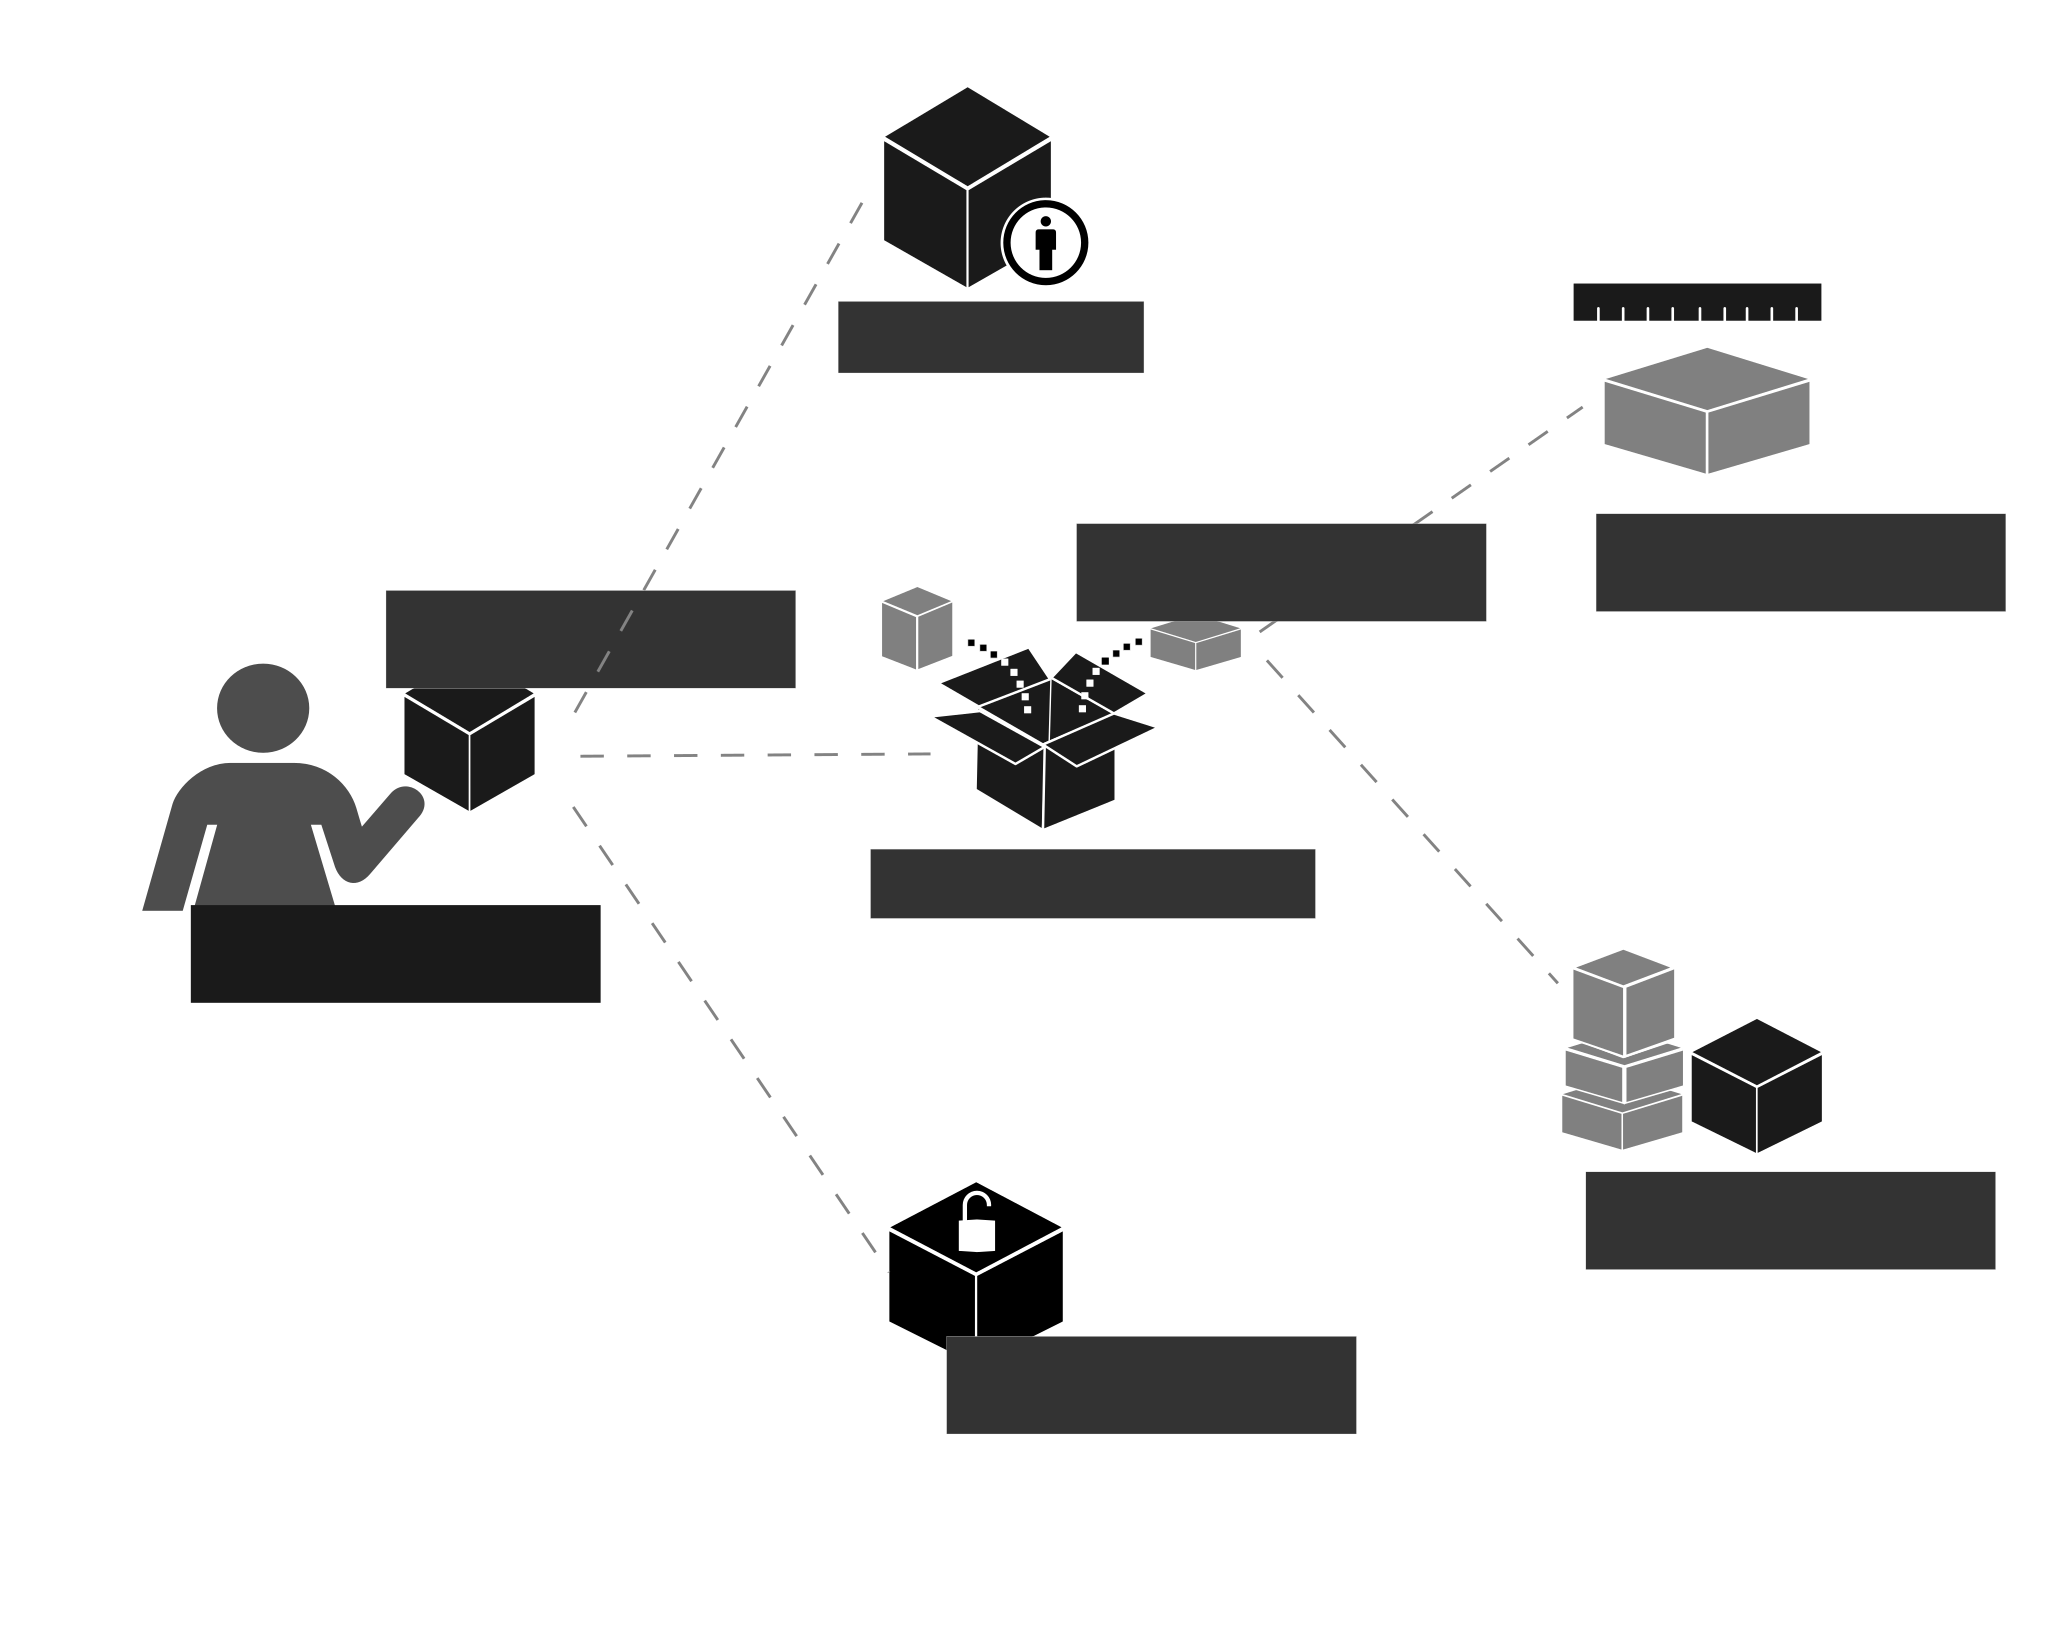
\includegraphics[width=3.25in]{figures/structure.pdf}
\caption{Structural dimensions of a remixing system}
\label{fig:structure}
\end{figure}



\section{Functional Role of Remixing}
I analyze the role remixing plays in participating in an online community of creators.
I look at how several forms of remixing are represented in the Scratch Online Community, how their use evolves, and how they do or do not support sociability and creative practices.
I analyze people's remixing behavior including their: 
1) adding to existing work, 
2) reusing components, 
3) collaborating with others in groups, 
4) persuading crowds to join remixing chains, 
5) inspiring others with ideas for new creations or 
6) self-appropriating their work to create something. 


\section{Attitudes Towards Remixing}
I investigate remixers' and originators' attitudes toward remixing, in particular, I analyze how participants use or perceive remixing as a cooperative or even 'antisocial' practice and how the system design may influence these attitudes. From the originator's perspective, I look at how and under what circumstances he or she reacts with: 
1) indifference, 
2) acceptance, 
3) encouragement, 
4) conditional acceptance or on an 
5) oppositional attitude. 
Similarly, I look at how remixers may go about remixing: 
1) obliviously, without regard to the norms, 
2) cautiously, or even 
3) antagonistically, as a form of trolling.
I explore these perspectives through case studies and by analyzing people's responses to design interventions intended to support proremixing attitudes and how failures to do so help inform future design repetitions. Analyzing these responses and attitudes can serve as a metric to understand the health of the community and to motivate further design interventions.

% Proposed research:
% How do young people respond to remixing? How are these attitudes represented in the community? When do they embrace remixing and when do they reject it?  I have and will analyze young people’s attitudes based on their own words (interviews) comments, reports (flags) and strategies for deterring (obfuscation, pseudo-licenses, Vigilantism) or supporting remixing (ommenting, scaffolding, framework approach, creation of narratives).
% Crowding out remixing by feaeturing
% Norms: plasticity of virtue
% Evolution of reactions as design changes




\chapter{Contributions}

Among the contributions of this thesis are:
\begin{itemize}
\item Conceptualization, design and implementation of a large online community of amateur creators.
\item Collection of a large corpus of research data that includes millions of interactive media projects and activity logs of more than half-a-million accounts.\footnote{Currently working on ways to release an anonymized version of these data to other researchers.}
\item A set of studies of sociotechnical design interventions.
\item A set of descriptive case studies of the activity on the Scratch Online Community.
\item A multidisciplinary framework to analyze and understand a new cultural phenomenon.
\end{itemize}

\section{Plan}

For the past four years, I have led the development of the Scratch website and worked on cultivating an online community that has grown to close to 800,000 people.
I have also published work describing the ways people participate, create, collaborate and remix on the Scratch Online Community \citep{monroy-hernandez_scratchr:_2007, monroy-hernandez_empowering_2008, monroy-hernandez_computers_2011, hill_responses_2010, aragon_tale_2009, nickerson_appropriation_2011, brennan_making_2010}.

Over the next few months, I plan to continue analyzing the structural, functional and attitudinal aspects of remixing in Scratch to better understand this specific phenomenon as well as the community at large.
I plan to integrate the findings into a cohesive framework for understanding remixing in a way that can be generalizable to other online remixing communities.

\subsection{Resources}
The technical infrastructure to support the website is in already in place.
In the coming days, I am planning to add two extra servers that will help further scale the website to handle more traffic and that will let me analyze the large corpus of data.
We also have a community manager, an IT consultant and a database specialist on a retainer who are able to assist with this research.
I already have the necessary approvals from COUHES\footnote{Committee On the Use of Humans as Experimental Subjects}.

\subsection{Timeline}
\begin{itemize}
\item May 2011 -- Data aggregation. In the first month, I plan to put together the data sets necessary to answer some research questions described in this document. Much of the data has already been collected, but it needs to be collated in an appropriate format for answering each question.
This phase is also exploratory, which will help tweak the framework in this proposal to better represent the patterns found in the data.
\item May 2011 -- Survey and experiment deployment. Also in the first month, I plan to deploy the necessary design interventions that will help get the necessary data that I do not have already. Most of these experiments are already programmed and just need to be tweaked.
\item June, July 2011 -- Data analysis. I plan to create the necessary visualizations and statistical analyses to examine some research questions outlined in this proposal. Additionally, I will build a set of representative case studies and execute the necessary interviews.
\item August 2011 -- Results. I plan to put together the findings in a structured form, and integrate all the findings into a cohesive document accessible to a broad audience.
\item September 2011 -- Draft -- a first draft of the dissertation.
\item January 2012 -- Defense\footnote{This date might change depending on whether whether I am in non-resident status or not}.
\item February 2012 -- Final version.
\end{itemize}

%Other chapters go here
%%Appendices
%\appendix
%Appendices go here. Structure is same as for other chapters
%%The bibliography
%\include{biblio}
\def\newblock{\hskip .11em plus .33em minus .07em}%not defined in the chi style
\bibliography{biblio}
\end{document}

%end file
